\section{Ejercicios}

\begin{enumerate}
\item Calcular las corrientes de malla mostradas en el circuito de la
  Figura \ref{fig.ejercicio2_tema1}.
  \begin{figure}[H]
    \centering 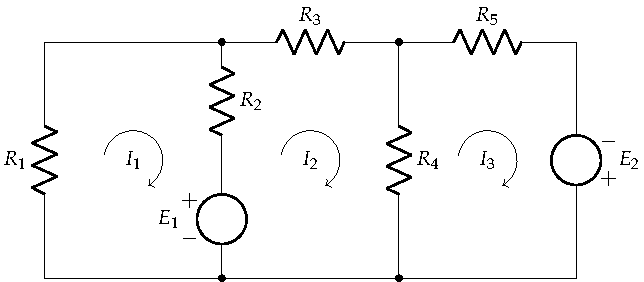
\includegraphics[height=3.7cm]{../figs/ej2_BT1.pdf}
    \caption{Ejercicio 1}
    \label{fig.ejercicio2_tema1}
  \end{figure}
  Datos: $R_1 = \qty{2}{\ohm}$; $R_2 = \qty{5}{\ohm}$; $R_3 = \qty{10}{\ohm}$, $R_4 = \qty{4}{\ohm}$; $R_5 = \qty{2}{\ohm}$; $E_1 = \qty{25}{\volt}$; $E_2 = \qty{50}{\volt}$

  \emph{Sol.: $I_1=-1.31$ A; $I_2=3.17$ A; $I_3=10.45$ A}
		
\item Calcular el valor de $E$ que hace que $I_0=7.5$ mA en el
  circuito de la Figura \ref{fig.ejercicio3_tema1}.
  \begin{figure}[H]
    \centering 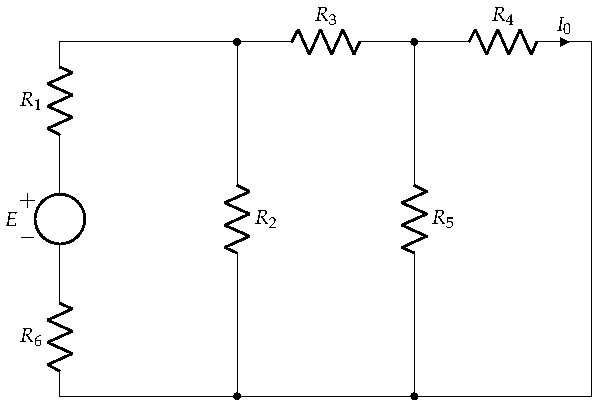
\includegraphics[height=5.5cm]{../figs/ej3_BT1.pdf}
    \caption{Ejercicio 2}
    \label{fig.ejercicio3_tema1}
  \end{figure}

  Datos: $R_1 = \qty{8}{\ohm}$; $R_2 = \qty{7}{\ohm}$; $R_3 = \qty{4}{\ohm}$, $R_4 = \qty{6}{\ohm}$; $R_5 = \qty{6}{\ohm}$; $R_6 = \qty{12}{\ohm}$; 

  \emph{Sol.: $U_s=0.705$ V}
		
\item Calcular la intensidad $I$ en el circuito de la Figura \ref{fig.ejercicio4_tema1}. \\
  \begin{figure}[H]
    \centering 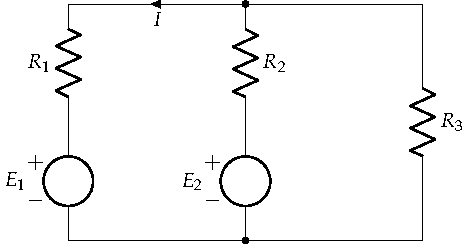
\includegraphics{../figs/ej4_BT1.pdf}
    \caption{Ejercicio 3}
    \label{fig.ejercicio4_tema1}
  \end{figure}
  Datos: $R_1 = \qty{27}{\ohm}$; $R_2 = \qty{47}{\ohm}$; $R_3 = \qty{27}{\ohm}$; $E_1 = \qty{460}{\volt}$; $E_2 = \qty{200}{\volt}$

  \emph{Sol.: $I=-8.77 $ A}
		
\item En el circuito de la Figura~\ref{fig.ejercicio8-bt1} obtener las
  intensidades de corriente señaladas primero mediante un análisis por
  el método de las mallas y posteriormente mediante un análisis por el
  método de los nudos.
  \begin{figure}[H]
    \centering 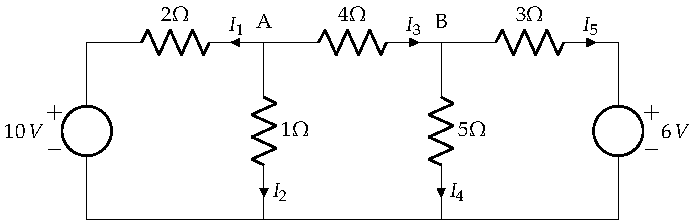
\includegraphics{../figs/ej8_BT1.pdf}
    \caption{Ejercicio 4}
    \label{fig.ejercicio8-bt1}
  \end{figure}

  Datos: $R_1 = \qty{2}{\ohm}$; $R_2 = \qty{1}{\ohm}$; $R_3 = \qty{4}{\ohm}$; $R_4 = \qty{5}{\ohm}$; $R_5 = \qty{3}{\ohm}$; $E_1 = \qty{10}{\volt}$; $E_2 = \qty{6}{\volt}$

  \emph{Sol.:
    $I_1=-3.31\,A;\;I_2=3.37\,{A};\; I_3=-0.06\,{A};\;
    I_4=0.73\,{A};\; I_5=-0.79\,A$}
 	
\item Analizar el circuito de la Figura~\ref{fig.mallas2} mediante el método de las mallas, obteniendo la corriente de cada una de las ramas. Con este resultado, calcular la diferencia de potencial entre A y B, y realizar un balance de potencias comparando la potencia de los elementos activos y la de los elementos pasivos. Datos: $R_1 = R_2 = {1}\Omega; R_3 = {2}\Omega; R_4 = {3}\Omega; R_5={4}\Omega; \epsilon_1={118} V; \epsilon_2 = 236V; \epsilon_3 = {118}V$.\\
  \begin{figure}[H]
    \centering 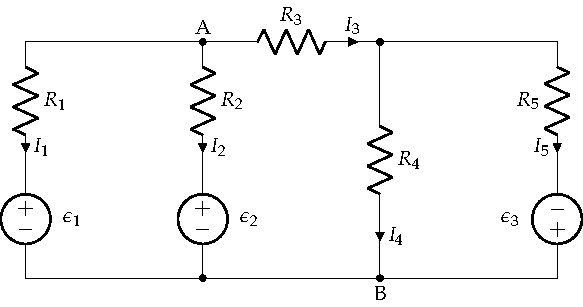
\includegraphics{../figs/mallas2.pdf}
    \caption{Ejercicio 5}
    \label{fig.mallas2}
  \end{figure}
  \emph{Sol.
    $I_1 = {32}A; I_2 = {-86} A; I_3 ={54}A; I_4 = {14}A; I_5 = {40}A;
    U_{AB}=150V; \sum P=0$}
 	
\item En el circuito de la Figura~\ref{fig.ej9_BT1}, determinar:
  \begin{itemize}
  \item Todas las intensidades de rama señaladas
  \item Carga, polaridad y energía almacenada en los condensadores
  \item Balance de potencias
  \end{itemize}
  \begin{figure}[H]
    \centering 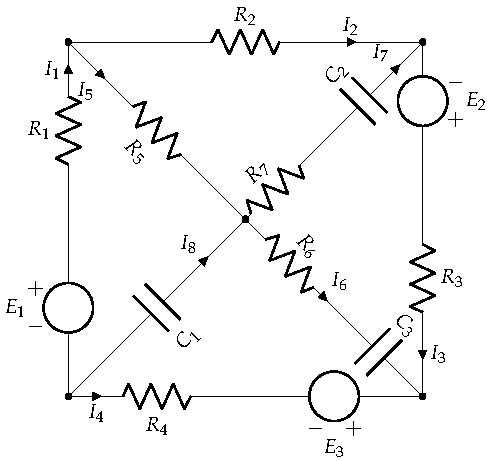
\includegraphics[height=6cm]{../figs/ej9_BT1.pdf}
    \caption{Ejercicio 6}
    \label{fig.ej9_BT1}
  \end{figure}
  Datos: $R_i = \qty[parse-numbers=false]{i}{\ohm}$; $C_i = \qty[parse-numbers=false]{i}{\micro\farad}$; $E_1 = \qty{8}{\volt}$; $E_2 = \qty{6}{\volt}$; $E_3 = \qty{4}{\volt}$

  \emph{Sol.:
    $I_1=I_2=I_3=-I_4=1\,A;\; I_5=I_6=I_7=0\,A;\;Q_{1\mu
      F}=-7\,\mu\text{C};\;Q_{2\mu F}=-4\,\mu\text{C};\;Q_{3\mu
      F}=3\,\mu\text{C};\;E_{1\mu F}=24.5\,\mu\text{J};\;E_{2\mu
      F}=4\,\mu\text{J};\; E_{3\mu F}=1.5\,\mu\text{J}$}
\item Aplicar el método de los nudos en el circuito de la
  Figura~\ref{fig.nudos_condensadores} para determinar:
  \begin{itemize}
  \item Los potenciales de los nudos A, B, C y D.
  \item Las intensidades de corriente señaladas.
  \item Carga, polaridad y energía almacenada en los condensadores,
    supuestos sin carga inicial.
  \end{itemize}
  Datos:
  $R_i = \mathrm{i\ } \Omega; C_i = \mathrm{i\ } \mu F; E_1 = 6V; E_2
  = 18 V; E_3 = {6} V$
  \begin{figure}[H]
    \centering 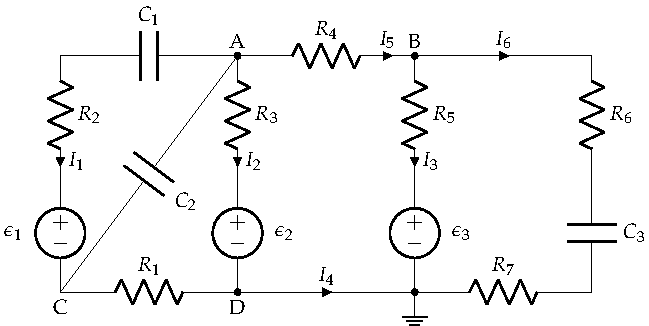
\includegraphics[]{../figs/nudos_condensadores.pdf}
    \caption{Ejercicio 7}
    \label{fig.nudos_condensadores}
  \end{figure}
  \emph{Sol.:
    $U_A=15V; U_B=11V; U_C=U_D=0V; I_1=I_6=0A;I_2=I_4=-1A; I_3=I_5=1A;
    q_1=9\mu C; q_2=30\mu C; q_3=33\mu C; E_{C1}=40.5\mu J;
    E_{C2}=225\mu J;E_{C2}=181.5\mu J$}

\item En el circuito de la Figura~\ref{fig.ej10_BT1}, donde se sabe
  que la carga inicial de los condensadores era de
  $\qty{10}{\micro\coulomb}$ para $C_1$ y de
  $\qty{20}{\micro\coulomb}$ para $C_2$ con las polaridades indicadas,
  se pide determinar:
  \begin{itemize}
  \item Intensidades de corriente señaladas
  \item Potenciales en los puntos A, B, C, D, E y F
  \end{itemize}

  Datos:
  $\epsilon_1=\SI{90}{\volt};\quad \epsilon_2=\SI{60}{\volt};\quad
  \epsilon_3=\SI{30}{\volt};\quad R_{1}= R_2 = R_3 =
  \SI{10}{\ohm};\quad R_{4}= R_5 = \SI{30}{\ohm};\quad C_{1}=
  \SI{10}{\micro\farad};\quad C_{2}= \SI{20}{\micro\farad};\quad L_1 =
  \SI{1}{\micro\henry}$

\begin{figure}[H]
  \centering 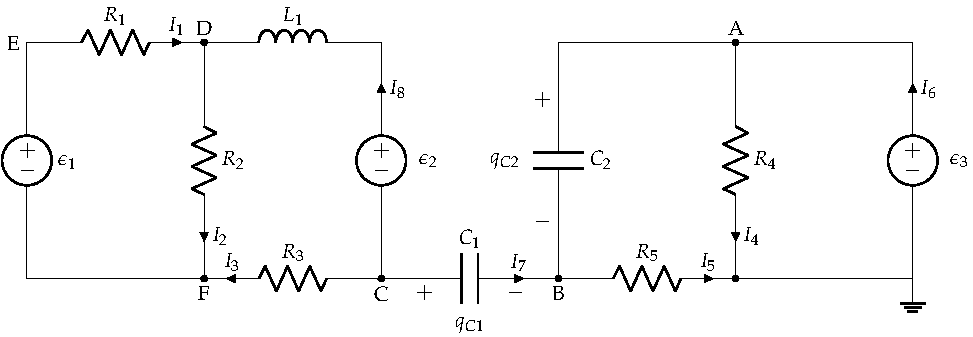
\includegraphics[scale =
  0.8]{../figs/mallas_carga_inicial.pdf}
  \caption{Ejercicio 8}
  \label{fig.ej10_BT1}
\end{figure}

\emph{Sol.
  $I_1=4A; I_2=5A; I_3=-1A;I_4=I_8=1A; I_5=I_7=0A; U_A=30V; U_B=0V;
  U_C=1V; U_D=61V;U_E=101V; U_F=11V$}

\item En el circuito de la Figura~\ref{fig.mallas_condensadores}, los
  condensadores se conectaron sin carga. Mediante el método de las
  mallas determina:
  \begin{itemize}
  \item Intensidades de corriente señaladas
  \item Potenciales en los puntos A, B, C y D
  \item Polaridades, cargas, y energías de los condensadores
  \item Balance de potencias
  \end{itemize}
  Datos:
  $ \epsilon_{1}={118}V; \epsilon_{2}={236} V; \epsilon_{3}=118V;
  R_{1}= {4}\Omega; R_{2}=R_{3}={1}{\Omega}; R_{4}= {3}{\Omega};
  R_{5}={2}{\Omega}; C_{1}=C_{2}=C_{3}={2}{\mu F}; X_1 = X_2 = X_3 =
  {1}{\Omega}$
  \begin{figure}[H]
    \centering 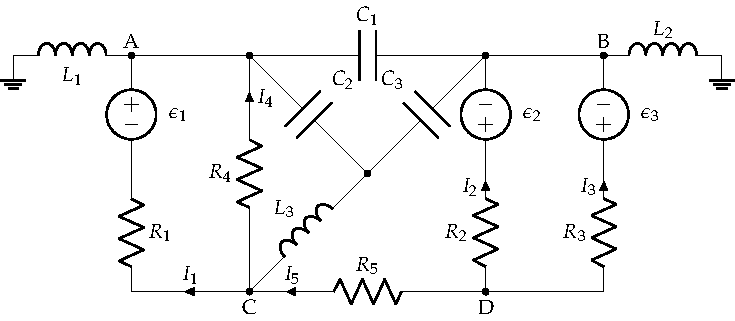
\includegraphics{../figs/mallas_condensadores.pdf}
    \caption{Ejercicio 9}
    \label{fig.mallas_condensadores}
  \end{figure}
  \emph{Sol.:
    $I_1=40A; I_2=-86A; I_3=32A; I_4=14A; I_5=54A; U_A=U_B=0V;
    U_C=41V; U_D=150V; U_{C1}=0V; q_1=0\mu F; E_{C1}=0J; U_{C2}=-42V;
    q_2=84\mu F; E_{C2}=1.76 mJ; U_{C3}=-42V; q_3=84\mu F; E_{C3}=1.76
    mJ; \sum P = 0$}

\item En el circuito de la Figura~\ref{fig.ej11_BT1}, determinar:
  \begin{itemize}
  \item Las ecuaciones para el cálculo de las intensidades
  \item Todas las intensidades indicadas
  \item Potenciales en todos los nudos
  \item Carga y energía almacenada en los condensadores
  \end{itemize}
  \begin{figure}[H]
    \centering 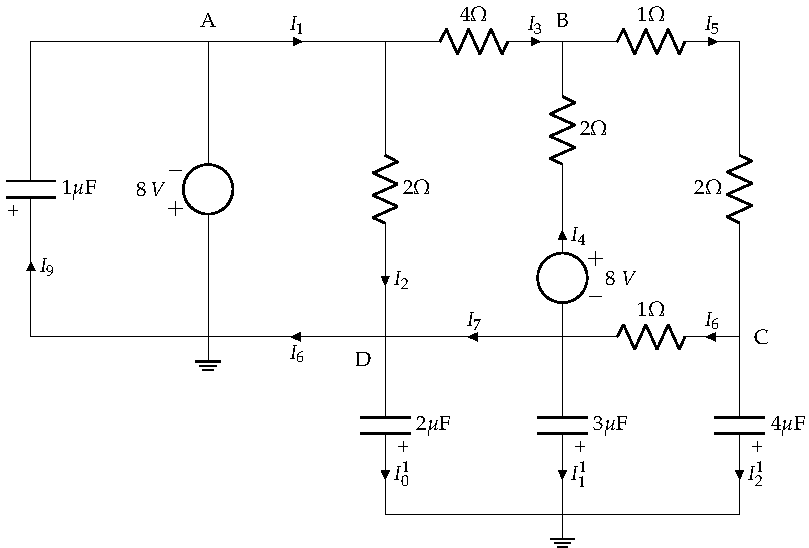
\includegraphics[height=8cm]{../figs/ej11_BT1.pdf}
    \caption{Ejercicio 10}
    \label{fig.ej11_BT1}
  \end{figure}

  Datos: $R_1 = \qty{2}{\ohm}$; $R_2 = \qty{4}{\ohm}$; $R_3 = \qty{2}{\ohm}$; $R_4 = \qty{1}{\ohm}$; $R_5 = \qty{2}{\ohm}$; $R_6 = \qty{1}{\ohm}$; $E_1 = \qty{8}{\volt}$; $E_2 = \qty{8}{\volt}$; $C_i = \qty[parse-numbers=false]{i}{\micro\farad}$

  \emph{Sol.:
    $I_1=I_6=-6.5A; I_2=-4A; I_3=-2.5A; I_4=3A; I_5=0.5A; U_A=-8V;
    U_B=2V; U_C=0.5V; U_D=0V;Q_{1\mu F}=8\mu C; Q_{2\mu F}=Q_{3\mu
      F}=0\mu C; Q_{4\mu F}=-2\mu C; E_{1\mu F}=32\mu F; E_{2\mu
      F}=E_{3\mu F}=0 J; E_{4\mu F}=0.5\mu C$}

\item En el circuito de la
  Figura~\ref{fig.mallas_agrupacion_condensadores} se debe determinar:
  \begin{itemize}
  \item Las corrientes señaladas.
  \item El balance de potencias, diferenciando entre elementos activos
    y elementos pasivos.
  \item Los potenciales en los puntos A, B y C.
  \item La carga y polaridad en los condensadores, supuestos sin carga
    inicial.
  \end{itemize}
  Datos:
  $\epsilon_1 ={1}V; \epsilon_2 ={7}V; R_i = {1}\Omega; C_i = {i}{\mu
    F}$
  \begin{figure}[H]
    \centering
    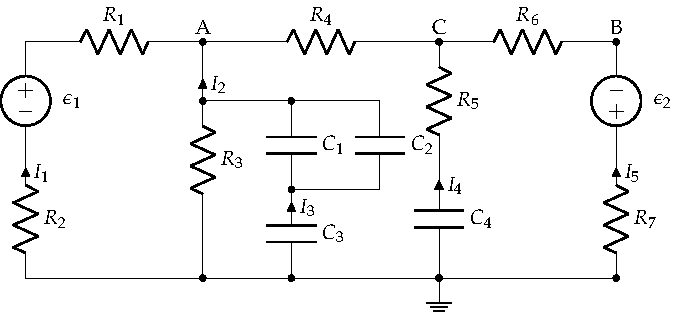
\includegraphics[height=5cm]{../figs/mallas_agrupacion_condensadores.pdf}
    \caption{Ejercicio 11}
    \label{fig.mallas_agrupacion_condensadores}
  \end{figure}
  \emph{Sol.:
    $I_1=I_2=1 A; I_3=I_4=0 A; I_5=-2 A; \sum P = 0; U_A=-1 V; U_B=-5
    V; U_C=-3 V; q_1=0.5 \mu C; q_2 = 1\mu F; q_3=1.5\mu F; q_4=12\mu
    C$}

\item El circuito de la Figura~\ref{fig.mallas_condensadores_bobinas}
  está funcionando en régimen estacionario. Los condensadores estaban
  inicialmente descargados. Resuelve el circuito mediante el método
  que consideres conveniente para obtener los siguientes resultados:
  \begin{itemize}
  \item Las intensidades señaladas.
  \item Polaridad y energía almacenada en los condensadores.
  \item Balance de potencias.
  \end{itemize}
  Datos:
  $\epsilon_{1}={40}V; \epsilon_{2}={22}V; \epsilon_{3}={20}V;
  C_{1}=C_{2}=C_{3}={2}{\mu F}; R_{g1}=R_{g2}=R_{g3}={4}{\Omega};
  R_{1}=R_{2}=R_{3}=R_{4}={2}{\Omega}; R_{5}=R_{6}=R_{7}={1}{\Omega}$
  \begin{figure}[H]
    \centering
    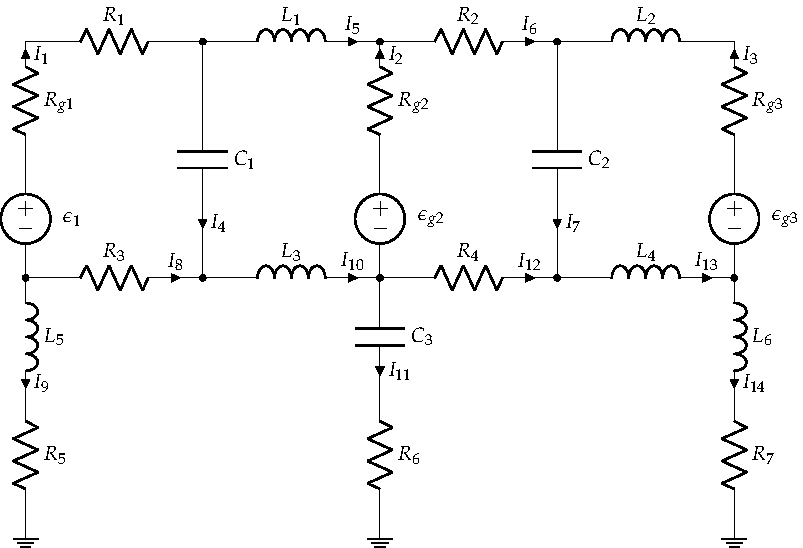
\includegraphics[height=8cm]{../figs/mallas_condensadores_bobinas.pdf}
    \caption{Ejercicio 12}
    \label{fig.mallas_condensadores_bobinas}
  \end{figure}
  \emph{Sol.:
    $I_1=I_5=2A; I_2=I_3=I_8=I_{10}=-1A;
    I_4=I_7=I_{11}=I_{12}=I_{13}=0A; I_6=I_{14}=1A; E_{C1}=0.676 mJ;
    E_{C2}=0.576 mJ; E_{C3}=1\mu J; \sum P = 0$}
 
\item En el circuito de la Figura~\ref{fig.ej12_BT1}, obtener las
  intensidades de corriente señaladas mediante un análisis por el
  método de las mallas y mediante un análisis por el método de los
  nudos.
  \begin{figure}[H]
    \centering 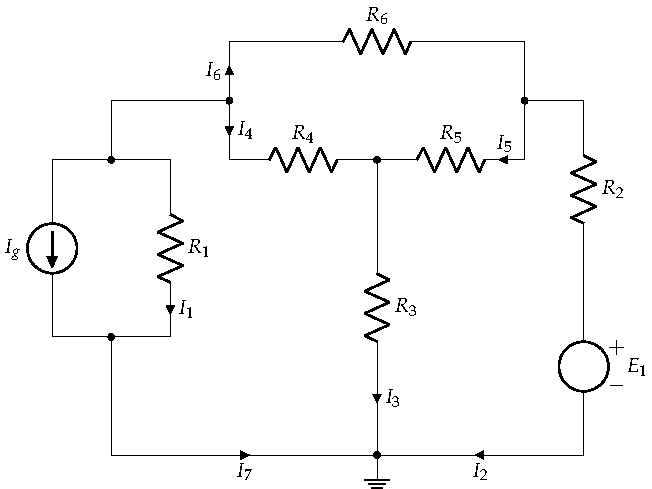
\includegraphics{../figs/ej12_BT1.pdf}
    \caption{Ejercicio 13}
    \label{fig.ej12_BT1}
  \end{figure}

    Datos: $R_1 = \qty{9}{\ohm}$; $R_2 = \qty{4}{\ohm}$; $R_3 = \qty{18}{\ohm}$; $R_4 = R_5 = R_6 = \qty{20}{\ohm}$; $E_1 = \qty{16}{\volt}$; $I_g = \qty{2}{\ampere}$

  \emph{Sol.:
    $I_1=-0.74\,A;\,I_2=-1.33\,A;\,I_3=0.07\,A;\,I_4=-0.39\,A;\;I_5=0.46\,A;\,I_6=-0.87\,A;\,I_7=1.26\,A$}

\item Calcular la intensidad que circula por la resistencia de 30
  $\Omega$ del circuito de la Figura~\ref{fig.ej16_BT1} aplicando el
  principio de superposición.
  \begin{figure}[H]
    \centering 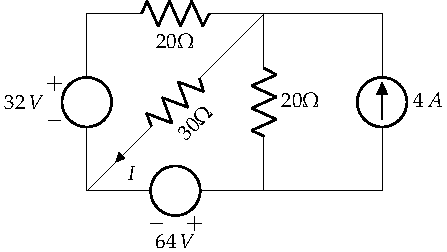
\includegraphics{../figs/ej16_BT1.pdf}
    \caption{Ejercicio 14}
    \label{fig.ej16_BT1}
  \end{figure}

  Datos: $R_1 = \qty{20}{\ohm}$; $R_2 = \qty{30}{\ohm}$; $R_3 = \qty{20}{\ohm}$; $E_1 = \qty{32}{\volt}$; $E_2 = \qty{64}{\volt}$; $I_g = \qty{4}{\ampere}$

  \emph{Sol.: $I=2.2\,A$}

\item Obtener el generador equivalente de Thévenin del circuito de la
  Figura~\ref{fig.ejTheveninRAB_BT1} respecto de A y B. A partir de
  este generador, calcula la resistencia a colocar en AB para obtener
  la máxima potencia, calculando esta potencia y la potencia entregada
  por el generador $\epsilon$.

  Datos:
  $\epsilon = \qty{54}{\volt};\quad R_1 = R_4 = \qty{8}{\ohm};\quad
  R_2 = R_3 = \qty{10}{\ohm}$

    \begin{figure}[H]
      \centering 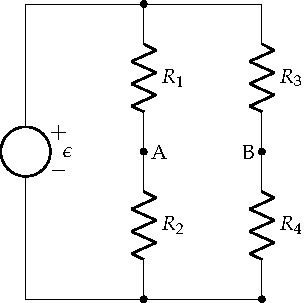
\includegraphics{../figs/Thevenin2}
      \caption{Ejercicio 15}
      \label{fig.ejTheveninRAB_BT1}
    \end{figure}

    \emph{Sol.:
      $R_{AB} = 80/9\si{\ohm}; \quad P_R = \qty{1.0125}{\watt}; \quad
      P_\epsilon = \qty{2.025}{\watt}$}

  \item Determinar el equivalente Thévenin del circuito de la
    Figura~\ref{fig.ej17_BT1} entre los nudos $A-B$. ¿Qué resistencia
    habría que conectar en dichos terminales para transferir la máxima
    potencia? ¿Cuál sería dicha potencia?
    \begin{figure}[H]
      \centering 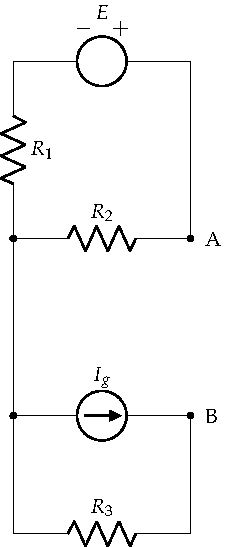
\includegraphics{../figs/ej17_BT1.pdf}
      \caption{Ejercicio 16}
      \label{fig.ej17_BT1}
    \end{figure}

    Datos: $R_1 = R_2 = \qty{4}{\ohm}$; $R_3 = \qty{2}{\ohm}$; $E = \qty{10}{\volt}$; $I_g = \qty{8}{\ampere}$

    \emph{Sol.:
      $\epsilon_{th}=5-16=-11\,V;\; R_{th}=4\Omega;\;
      R_L=4\Omega;\;P_{max}=7.56$ W}


  \item Obtener el generador equivalente de Thévenin del circuito de la Figura~\ref{fig.ej18_BT1} respecto de A y B.\\
    Datos: $I_g=10\,A; R_1=1\Omega;\; \alpha=5$
    \begin{figure}[H]
      \centering 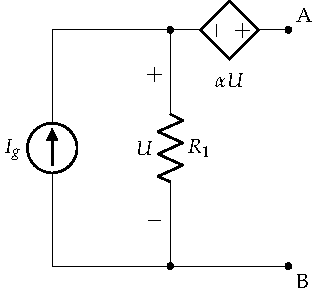
\includegraphics[height=4.5cm]{../figs/Thevenin1.pdf}
      \caption{Ejercicio 17}
      \label{fig.ej18_BT1}
    \end{figure}
    \emph{Sol.: $\epsilon_{th}=60\,V;\;R_{th}=6\Omega$}

  \item En el circuito de la Figura~\ref{fig.norton_ej}, calcular:
    \begin{itemize}
    \item La corriente del generador equivalente de Norton respecto de
      A y B, $I_N$.
    \item La resistencia del generador equivalente de Norton respecto
      de A y B, $R_N$.
    \item La resistencia de carga que se debe conectar entre A y B
      para conseguir la máxima potencia disponible, y el valor de esta
      potencia.
    \end{itemize}

    Datos:
    $R = {1}{\Omega};\; \epsilon_g = {10}{V};\; \alpha = \beta = 1$

\begin{figure}[H]
  \centering 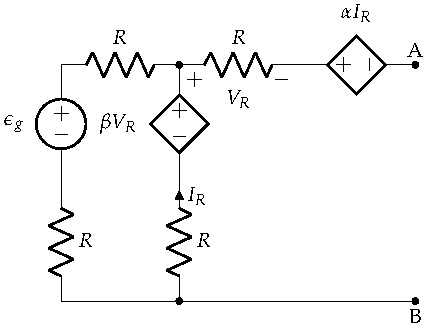
\includegraphics[height=4.5cm]{../figs/norton.pdf}
  \caption{Ejercicio 18}
  \label{fig.norton_ej}
\end{figure}

\emph{Sol.:
  $I_N=\frac{10}{3}\,A;\; R_N=2\,\Omega;\; R_L=2\Omega;\;
  P_L=5.56\,W$}


% \begin{remark}
%   Los ejercicios 19 y 20 constituyen contenido avanzado.
% \end{remark}

% \item Determinar las corrientes marcadas en la
%   Figura~\ref{fig.ej13_BT1}.
%   \begin{figure}[H]
%     \centering 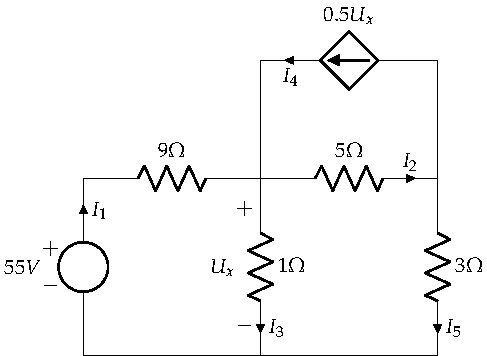
\includegraphics[height=5cm]{../figs/ej13_BT1.pdf}
%     \caption{Ejercicio 19}
%     \label{fig.ej13_BT1}
%   \end{figure}
%   \emph{Sol.:
%
%
%
%
%
%
%
%
%
%
%
%
%
%
%
%
%
%
%
%
%
%
%
%
%
%
%
%
%
%
%
%
%
%
%
%
%
%
%
%
%
%
%
%
%
%
%
%
%
%
%
%
%
%
%
%
%
%
%
%
%
%
%
%
%
%
%
%
%
%
%
%
%
%
%
%
%
%
%
%
%
%
%
%
%
%
%
%
%
%
%
%
%
%
%
%
%
%
%
%
%
%
%
%
%
%
%
%
%
%
%
%
%
%
%
%
%
%
%
%
%
%
%
%
%
%
%
%
%
%
%
%
%
%
%
%
%
%
%
%
%
%
%
%
%
%
%
%
%
%
%
%
%
%
%
%
%
%
%
%
%
%
%
%
%
%
%
%
%
%
%
%
%
%
%
%
%
%
%
%
%
%
%
%
%
%
%
%
%
%
%
%
%
%
%
%
%
%
%
%
%
%
%
%
%
%
%
%
%
%
%
%
%
%
%
%
%
%
%
%
%
%
%
%
%
%
%
%
%
%
%
%
%
%
%
%
%
%
%
%
%
%
%
%
%
%
%
%
%
%
%
%
%
%
%
%
%
%
%
%
%
%
%
%
%
%
%
%
%
%
%
%
%
%
%
%
%
%
%
%
%
%
%
%
%
%
%
%
%
%
%
%
%
%
%
%
%
%
%
%
%
%
%
%
%
%
%
%
%
%
%
%
%
%
%
%
%
%
%
%
%
%
%
%
%
%
%
%
%
%
%
%
%
%
%
%
%
%
%
%
%
%
%
%
%
%
%
%
%
%
%
%
%
%
%
%
%
%
%
%
%
%
%
%
%
%
%
%
%
%
%
%
%
%
%
%
%
%
%
%
%
%
%
%
%
%
%
%
%
%
%
%
%
%
%
%
%
%
%
%
%
%
%
%
%
%
%
%
%
%
%
%
%
%
%
%
%
%
%
%
%
%
%
%
%
%
%
%
%
%
%
%
%
%
%
%
%
%
%
%
%
%
%
%
%
%
%
%
%
%
%
%
%
%
%
%
%
%
%
%
%
%
%
%
%
%
%
%
%
%
%
%
%
%
%
%
%
%
%
%
%
%
%
%
%
%
%
%
%
%
%
%
%
%
%
%
%
%
%
%
%
%
%
%
%
%
%
%
%
%
%
%
%
%
%
%
%
%
%
%
%
%
%
%
%
%
%
%
%
%
%
%
%
%
%
%
%
%
%
%
%
%
%
%
%
%
%
%
%
%
%
%
%
%
%
%
%
%
%
%
%
%
%
%
%
%
%
%
%
%
%
%
%
%
%
%
%
%
%
%
%
%
%
%
%
%
%
%
%
%
%
%
%
%
%
%
%
%
%
%
%
%
%
%
%
%
%
%
%
%
%
%
%
%
%
%
%
%
%
%
%
%
%
%
%
%
%
%
%
%
%
%
%
%
%
%
%
%
%
%
%
%
%
%
%
%
%
%
%
%
%
%
%
%
%
%
%
%
%
%
%
%
%
%
%
%
%
%
%
%
%
%
%
%
%
%
%
%
%
%
%
%
%
%
%
%
%
%
%
%
%
%
%
%
%
%
%
%
%
%
%
%
%
%
%
%
%
%
%
%
%
%
%
%
%
%
%
%
%
%
%
%
%
%
%
%
%
%
%
%
%
%
%
%
%
%
%
%
%
%
%
%
%
%
%
%
%
%
%
%
%
%
%
%
%
%
%
%
%
%
%
%
%
%
%
%
%
%
%
%
%
%
%
%
%
%
%
%
%
%
%
%
%
%
%
%
%
%
%
%
%
%
%
%
%
%
%
%
%
%
%
%
%
%
%
%
%
%
%
%
%
%
%
%
%
%
%
%
%
%
%
%
%
%
%
%
%
%
%
%
%
%
%
%
%
%
%
%
%
%
%
%
%
%
%
%
%
%
%
%
%
%
%
%
%
%
%
%
%
%
%
%
%
%
%
%
%
%
%
%
%
%
%
%
%
%
%
%
%
%
%
%
%
%
%
%
%
%
%
%
%
%
%
%
%
%
%
%
%
%
%
%
%
%
%
%
%
%
%
%
%
%
%
%
%
%
%
%
%
%
%
%
%
%
%
%
%
%
%
%
%
%
%
%
%
%
%
%
%
%
%
%
%
%
%
%
%
%
%
%
%
%
%
%
%
%
%
%
%
%
%
%
%
%
%
%
%
%
%
%
%
%
%
%
%
%
%
%
%
%
%
%
%
%
%
%
%
%
%
%
%
%
%
%
%
%
%
%
%
%
%
%
%
%
%
%
%
%
%
%
%
%
%
%
%
%
%
%
%
%
%
%
%
%
%
%
%
%
%
%
%
%
%
%
%
%
%
%
%
%
%
%
%
%
%
%
%
%
%
%
%
%
%
%
%
%
%
%
%
%
%
%
%
%
%
%
%
%
%
%
%
%
%
%
%
%
%
%
%
%
%
%
%
%
%
%
%
%
%
%
%
%
%
%
%
%
%
%
%
%
%
%
%
%
%
%
%
%
%
%
%
%
%
%
%
%
%
%
%
%
%
%
%
%
%
%
%
%
%
%
%
%
%
%
%
%
%
%
%
%
%
%
%
%
%
%
%
%
%
%
%
%
%
%
%
%
%
%
%
%
%
%
%
%
%
%
%
%
%
%
%
%
%
%
%
%
%
%
%
%
%
%
%
%
%
%
%
%
%
%
%
%
%
%
%
%
%
%
%
%
%
%
%
%
%
%
%
%
%
%
%
%
%
%
%
%
%
%
%
%
%
%
%
%
%
%
%
%
%
%
%
%
%
%
%
%
%
%
%
%
%
%
%
%
%
%
%
%
%
%
%
%
%
%
%
%
%
%
%
%
%
%
%
%
%
%
%
%
%
%
%
%
%
%
%
%
%
%
%
%
%
%
%
%
%
%
%
%
%
%
%
%
%
%
%
%
%
%
%
%
%
%
%
%
%
%
%
%
%
%
%
%
%
%
%
%
%
%
%
%
%
%
%
%
%
%
%
%
%
%
%
%
%
%
%
%
%
%
%
%
%
%
%
%
%
%
%
%
%
%
%
%
%
%
%
%
%
%
%
%
%
%
%
%
%
%
%
%
%
%
%
%
%
%
%
%
%
%
%
%
%
%
%
%
%
%
%    $I_1=I_a=5.38\,A;\;I_2=2.07\,A; I_3=6.62\,A\; I_4=3.31\,A\; I_5=-1.24\,A$}

% \item Determinar las tensiones en los nudos $A$ y $B$ del circuito de la Figura~\ref{fig.ej14_BT1}.
% \begin{figure}[H]
%     \centering
%     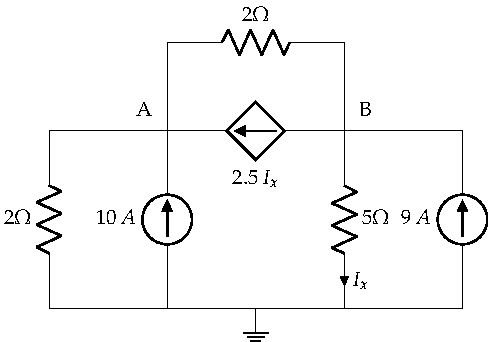
\includegraphics[height=5cm]{../figs/ej14_BT1.pdf}
%     \caption{Ejercicio 20}
%     \label{fig.ej14_BT1}
% \end{figure}
% \emph{Sol.: $U_A=30\,V;\;U_B=20\,V$}

\end{enumerate}

%%% Local Variables:
%%% mode: latex
%%% TeX-master: "enunciados_ejercicios_TC"
%%% ispell-local-dictionary: "castellano"
%%% End:
